\documentclass[12pt]{article}

\usepackage{geometry}
\geometry{a4paper, left=1in, right=1in, top=1in, bottom=1in}
\usepackage{amsmath}
\usepackage{amsmath,amsfonts,amssymb}
\usepackage{graphicx}
\usepackage{enumitem}
\usepackage{titlesec}
\usepackage{fancyhdr}
\usepackage{hyperref}
\usepackage{floatrow}
\title{CS663 Assignment 1}
\author{Saksham Rathi, Kavya Gupta, Shravan Srinivasa Raghavan}
\begin{document}
\maketitle
\clearpage
\tableofcontents
\clearpage
\section*{Question 1}

In the first scenario, both the images differ in the pixel resolution but maintain the same aspect ratio (square pixels). We will use the motion model with the following features:
\begin{itemize}
    \item Translation: To align the images based on the control points
    \item Rotation: To correct any angular misalignment between the images.
    \item Uniform Scaling: To account for the difference in pixel sizes (since both images have square pixels, the scaling factor will be uniform).
\end{itemize}
Such a transformation is sufficient in this case, because we don't need non-uniform scaling (both the pixels are square) and shearing.


In the second scenario, both the images have different pixel shapes (the second one is rectangular). We will have to use affine transformation in this case:
\begin{itemize}
    \item Translation: To align the images based on the control points
    \item Rotation: To correct any angular misalignment between the images.
    \item Non-uniform Scaling: To account for the different scaling factors in the x and y directions.
    \item Shearing: To correct skewness.
\end{itemize}
This model can handle non-uniform scaling and shearing along with the features in the previous scenario, making it suitable aligning images with different pixel sizes.
\clearpage
\section*{Question 2}

    \vspace{-10pt}

    \subsection*{Relationship between the motion vectors}

    \vspace{-5pt}

    It can be understood as follows:

    Given that the motion is purely translational:

    \vspace{-10pt}

    \begin{itemize}[itemsep=-0.25em]
        \item $u_{12}$ represents the motion vector that aligns image $I_2$ with image $I_1$.
        \item $u_{23}$ represents the motion vector that aligns image $I_3$ with image $I_2$.
        \item $u_{13}$ represents the motion vector that aligns image $I_3$ with image $I_1$.
    \end{itemize}

    \vspace{-9pt}

    The relationship between these motion vectors can be described using vector addition:

    \vspace{-10pt}

    \[
    u_{13} = u_{12} + u_{23}
    \]

    This equation means that to align $I_3$ with $I_1$, you can first align $I_3$ with $I_2$ using $u_{23}$, and then align $I_2$ with $I_1$ using $u_{12}$.

    \vspace{-10pt}

    \subsection*{Practical Consideration}

    \vspace{-5pt}

    In an ideal scenario (i.e., perfect conditions with no noise, distortion, or errors), this relationship would hold exactly in practice.\ However, in real-world applications, some distorting factor (most likely to be present in practical estimation) may cause this relationship to not hold.

    \vspace{-10pt}

    \begin{enumerate}[itemsep=-0.25em]
        \item \textbf{Noise:} Image data is often noisy due to sensor imperfections, lighting variations, or other environmental factors. This noise can lead to inaccuracies in the estimation of the motion vectors.
        \item \textbf{Numerical Precision:} Computational limitations such as numerical precision and rounding errors can also introduce small deviations from the expected relationship.
        \item \textbf{Pixels:} This motion between the images isn’t completely continuous i.e. it’s discrete, limited by the pixel size. Hence if the actual motion is having some fractional term (in terms of pixels), we have to round it up/down causing devation from the relationship.
    \end{enumerate}
    \clearpage
\section*{Question 3}

    \begin{itemize}
        \item Since we have access to the coordinates of both MATLAB's coordinate system and that of the image, we can compute the 
        transformation matrix between the two coordinate systems. Since the graph is not rotated, the equations are fairly 
        simple.
        \item The only possible relative motions are shifting of the orgin and non uniform scaling.
    \end{itemize}

    Therefore we have 
    \begin{align}
        \begin{pmatrix}
            x_{2} \\
            y_{2} \\
            1
        \end{pmatrix}
        = \mathcal{T} 
        \begin{pmatrix}
            x_{1} \\
            y_{1} \\
            1
        \end{pmatrix}
    \end{align}
    where $\mathcal{T} = \begin{pmatrix}
                            c_{1} & 0 & t_{x} \\
                            0  & c_{2} & t_{y} \\
                            0 & 0 & 1
                        \end{pmatrix}$

    The transformation represented by $\mathcal{T}$ can be solved for step by step by taking a few points from the image 
    and mapping with the coordinates in MATLAB's graph. First step would be to solve for the origins of both the systems.
    This would give us the values of $t_{x}$ and $t_{y}$. Then once that is done, we can compare the scales of both 
    the systems. The scales are basically the values $c_{1}$ and $c_{2}$ and we are done.
\clearpage
\section*{Question 4}

    \begin{itemize}
        \item There are $12$ unknown parameters $A,B,C,D,E,F,a,b,c,d,e$ and $f$, therefore we would need at least $12/2 = 6$ 
        control points.
        \item Let the pairs of physically corresponding control points be $\{(x_{11},y_{11}),(x_{21},y_{21})\}$, 
        $\{(x_{12},y_{12}),(x_{22},y_{22})\}$, $\{(x_{13},y_{13}),(x_{23},y_{23})\}$, $\{(x_{14},y_{14}),(x_{24},y_{24})\}$.
        $\{(x_{15},y_{15}),(x_{25},y_{25})\}$ and $\{(x_{16},y_{16}),(x_{26},y_{26})\}$.
    \end{itemize}
    We are given that for any pair of
    corresponding points $\{(x_{1},y_{1}),(x_{2},y_{2})\}$ the motion model is
    \begin{align}
        \label{main}
        \begin{pmatrix}
            x_{2} \\
            y_{2}
        \end{pmatrix}
        =
        \begin{pmatrix}
            a & b & c & d & e & f \\
            A & B & C & D & E & F
        \end{pmatrix}
        \cdot
        \begin{pmatrix}
            x_{1}^{2} \\
            y_{1}^{2} \\
            x_{1}y_{1} \\
            x_{1} \\
            y_{1} \\
            1
        \end{pmatrix}
    \end{align}
    For each pair of control points that we have taken, there would be an equation similar to \ref{main}. The general format
    would look like this 
    \begin{align}
        \label{spec}
        \begin{pmatrix}
            x_{2k} \\
            y_{2k}
        \end{pmatrix}
        =
        \begin{pmatrix}
            a & b & c & d & e & f \\
            A & B & C & D & E & F
        \end{pmatrix}
        \cdot
        \begin{pmatrix}
            x_{1k}^{2} \\
            y_{1k}^{2} \\
            x_{1k}y_{1k} \\
            x_{1k} \\
            y_{1k} \\
            1
        \end{pmatrix}        
    \end{align}
    where $k \in \{1,2,3,4,5,6\}$. 

    Combining all 6 eqautions we get, 
    \begin{align}
        \label{final1}
        \begin{pmatrix}
            x_{21} & x_{22} & x_{23} & x_{24} & x_{25} & x_{26}\\
            y_{21} & y_{22} & y_{23} & y_{24} & y_{25} & y_{26}
        \end{pmatrix}
        &
        =
        \begin{pmatrix}
            a & b & c & d & e & f \\
            A & B & C & D & E & F
        \end{pmatrix}
        \cdot 
        \nonumber \\
        &\begin{pmatrix}
            x_{11}^{2} & x_{12}^{2} & x_{13}^{2} & x_{14}^{2} & x_{15}^{2} & x_{16}^{2} \\
            y_{11}^{2} & y_{12}^{2} & y_{13}^{2} & y_{14}^{2} & y_{15}^{2} & y_{16}^{2} \\
            x_{11}y_{11} & x_{12}y_{12} & x_{13}y_{13} & x_{14}y_{14} & x_{15}y_{15} & x_{16}y_{16} \\
            x_{11} & x_{12} & x_{13} & x_{14} & x_{15} & x_{16} \\
            y_{11} & y_{12} & y_{13} & y_{14} & y_{15} & y_{16} \\ 
            1 & 1 & 1 & 1 & 1 & 1 
        \end{pmatrix}        
    \end{align}
    Let $X_{2} = \begin{pmatrix}
        x_{21} & x_{22} & x_{23} & x_{24} & x_{25} & x_{26}\\
        y_{21} & y_{22} & y_{23} & y_{24} & y_{25} & y_{26}
    \end{pmatrix}$, $X_{1} = \begin{pmatrix}
        x_{11}^{2} & x_{12}^{2} & x_{13}^{2} & x_{14}^{2} & x_{15}^{2} & x_{16}^{2} \\
        y_{11}^{2} & y_{12}^{2} & y_{13}^{2} & y_{14}^{2} & y_{15}^{2} & y_{16}^{2} \\
        x_{11}y_{11} & x_{12}y_{12} & x_{13}y_{13} & x_{14}y_{14} & x_{15}y_{15} & x_{16}y_{16} \\
        x_{11} & x_{12} & x_{13} & x_{14} & x_{15} & x_{16} \\
        y_{11} & y_{12} & y_{13} & y_{14} & y_{15} & y_{16} \\ 
        1 & 1 & 1 & 1 & 1 & 1 
    \end{pmatrix}$
    and $\mathcal{M} = \begin{pmatrix}
        a & b & c & d & e & f \\
        A & B & C & D & E & F
    \end{pmatrix} $. Equation \ref{final1} can be written compactly as 
    \begin{align}
        X_{2} = \mathcal{M} \cdot X_{1} \nonumber \\
        \Rightarrow \boxed{\label{final2} \mathcal{M} = X_{2} \cdot X_{1}^{-1}} 
    \end{align}
    Therefore selecting control points such $X_{1}$ is invertible and solving equation \ref{final2} will provide the 
    matrix $\mathcal{M}$ whose entries are the constants $A,B,C,D,E,F,a,b,c,d,e$ and $f$.
    \clearpage
    \section*{Question 5}

    \vspace{-10pt}
    
    \textbf{(a)} The code is in \verb|Code/Q5_Code.m| and the rotated image is \verb|Images/Q5/T2_rotated.jpg|. \newline
    \textbf{(b)} The code is in \verb|Code/Q5_Code.m|. \newline
    \textbf{(c)} Here are the graphs:-
    
    \vspace{-13pt}
    
    \begin{figure}[H]
        \centering
        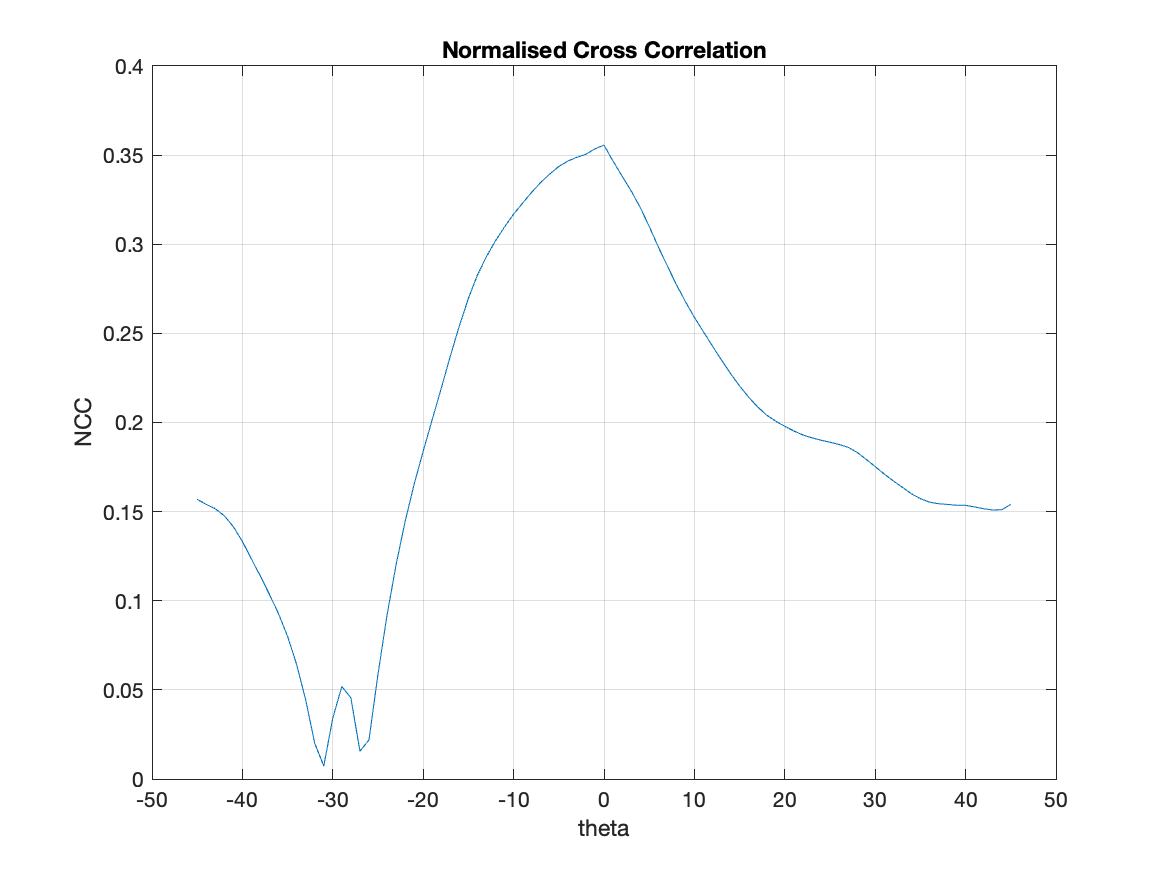
\includegraphics[width=0.59\textwidth]{Images/Q5/NCC.png}
        \vspace{-10pt}
        \caption{Normalised Cross Correlation (NCC) v/s $\theta$}
    \end{figure}
    
    \vspace{-25pt}
    
    \begin{figure}[H]
        \centering
        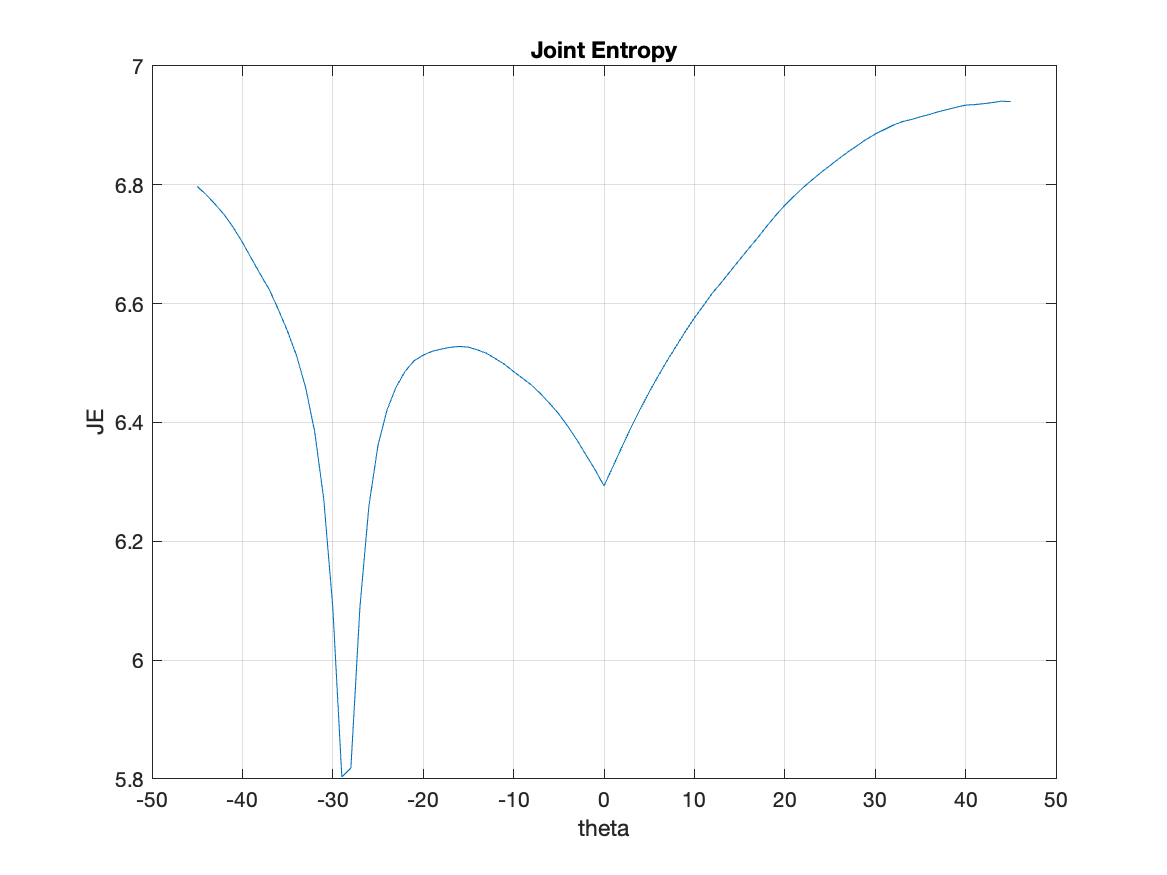
\includegraphics[width=0.59\textwidth]{Images/Q5/JE.png}
        \vspace{-10pt}
        \caption{Joint Entropy (JE) v/s $\theta$}
    \end{figure}
    
    \vspace{-25pt}
    
    \begin{figure}[H]
        \centering
        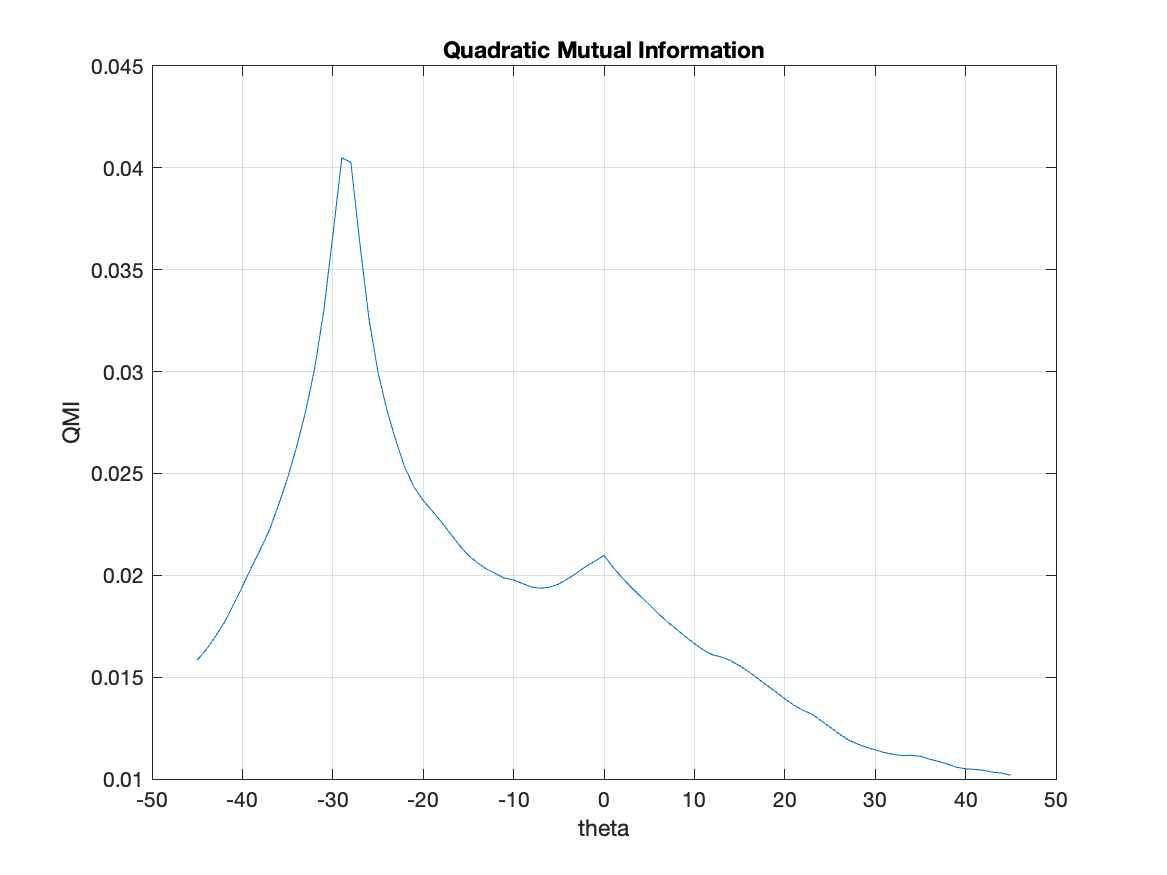
\includegraphics[width=0.59\textwidth]{Images/Q5/QMI.png}
        \vspace{-10pt}
        \caption{Quadratic Mutual Information (QMI) v/s $\theta$}
    \end{figure}
    
    \textbf{(d)} Here are some observations:-
    
    \vspace{-10pt}
    
    \begin{itemize}[itemsep=0em]
        \item \textbf{NCC:} More the absolute value of NCC, better the linear relation between the images. Global maxima exists at $\theta = 0^{\circ}$, which is clearly not the correct rotation. There does exist a local maxima at around $\theta = -29^{\circ}$ which we wanted. Hence it can be observed that NCC is not a good measure always to deal with image alignment.
        \item \textbf{JE:} Lesser the JE, better the alignment. We see that the global minima exists at $\theta = -29^{\circ}$, close to our expected value ($28.5^{\circ}$ clockwise) upto precision of 1 degree, given the step size of theta is 1 degree too. Hence, JE checks out to be a good method for checking image alignment. We also observe a local minima at $\theta = 0^{\circ}$.
        \item \textbf{QMI:} More the QMI, better the alignment. We see that the global maxima exists at $\theta = -29^{\circ}$, close to our expected value ($28.5^{\circ}$ clockwise) upto precision of 1 degree, given the step size of theta is 1 degree too. Hence, QMI checks out to be a good method for checking image alignment. We also observe a local maxima at $\theta = 0^{\circ}$.
    \end{itemize}
    
    \vspace{-10pt}
    
    Here are the optimal rotations:-
    
    \vspace{-10pt}
    
    \begin{table}[H]
        \centering
        \begin{tabular}{|c|c|}
            \hline
            Measure & Optimal $\theta$ \\
            \hline
            NCC & $0^{\circ}$ \\
            JE & $-29^{\circ}$ \\
            QMI & $-29^{\circ}$ \\
            \hline
        \end{tabular}
    \end{table}
    
    \vspace{-10pt}
    
    \textbf{(e)} The code is in \texttt{Q5\_Code.m} and the joint histogram for $\theta = -29^{\circ}$:-
    
    \vspace{-13pt}
    
    \begin{figure}[H]
        \centering
        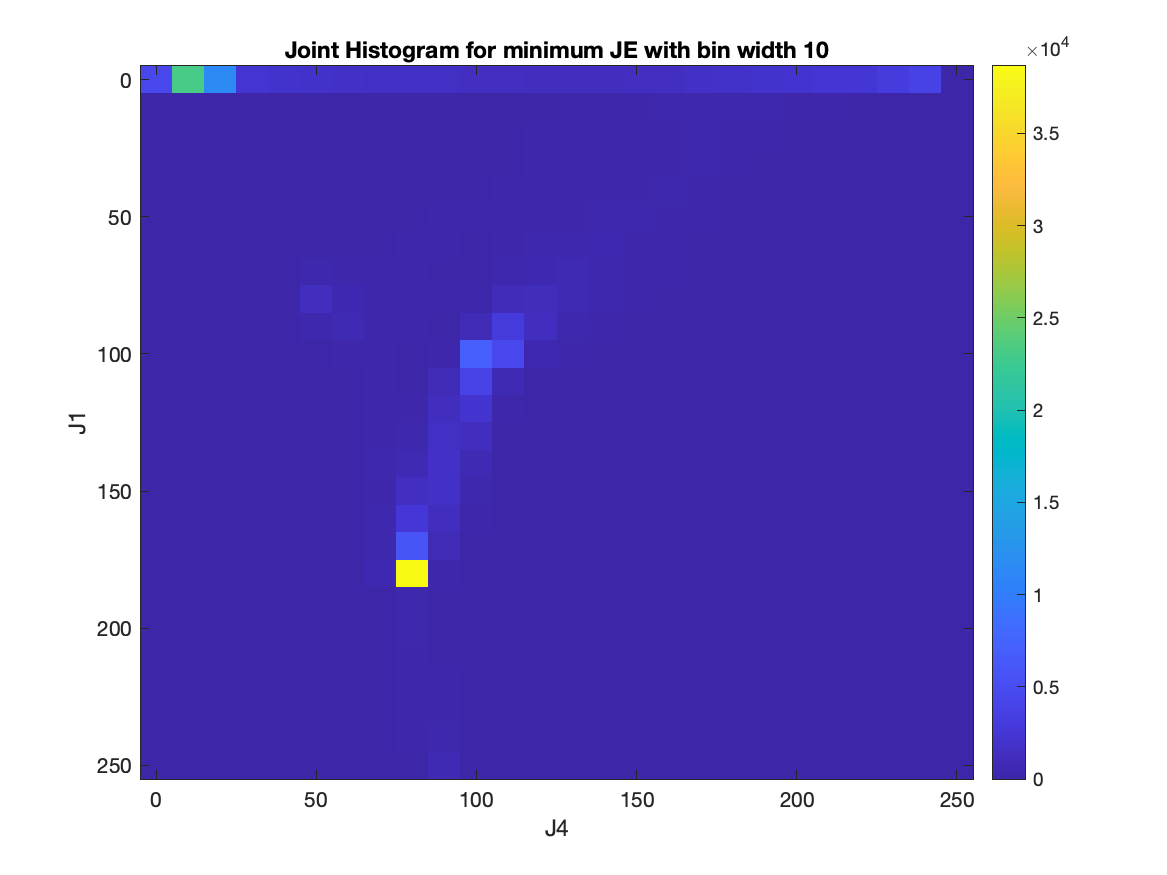
\includegraphics[width=0.59\textwidth]{Images/Q5/Joint_hist_JE.png}
        \vspace{-10pt}
        \caption{Joint Histogram for $\theta = -29^{\circ}$}
    \end{figure}
    
    \vspace{-10pt}

    \textbf{(f)} When two discrete random variables $I_1$ and $I_2$ are statistically independent, then $p_{I_1 I_2}(i_1,i_2)=p_{I_1}(i_1) \times p_{I_2}(i_2) \; \forall \; i_1, i_2$ (in domain of the variables), i.e. joint PMF is equal to product of the marginal PMFs. In that case, QMI would be equal to $0$. Hence the more the difference between $p_{I_1 I_2}(i_1,i_2)$ and $p_{I_1}(i_1) \times p_{I_2}(i_2)$, the more dependent the variables are. Hence the more aligned (correlated) the images are, QMI tends to be higher. Hence images are aligned when QMI is maximum.
    
    Also unlike NCC, QMI can detect non-linear relation between variables.
\clearpage
\section*{Question 6}
\textbf{(a)} The images were read using the imread function (and cast as double). Then we took 12 pairs of point as input from the user (through mouse click). The points were choosen to be as accurate and similar as possible. The values were saved in ``selected\_points.mat" to save effort for further runs. Here is a small section of the code:
\begin{verbatim}
n = 12; % Number of points
for i=1:n
    figure(1); 
    imshow(im1/255); 
    [x1(i), y1(i)] = ginput(1);
    figure(2); 
    imshow(im2/255); 
    [x2(i), y2(i)] = ginput(1);
end
save(`selected_points.mat', `x1', `y1', `x2', `y2');
\end{verbatim}


\textbf{(b)}
We consider that the affine transformation matrix will be of the form:
\[
    \begin{bmatrix}
        x_1 & x_2 & x_3 \\
        x_4 & x_5 & x_6 \\
        0 & 0 & 1
    \end{bmatrix}
\]

We initialize matrix A with points from Img1 (n = 12 in our case):
\[
    \begin{bmatrix}
        x_{11} & x_{12} & x_{13} & \dots & x_{1n} \\
        y_{11} & x_{12} & y_{13} & \dots & y_{1n} \\
        1 & 1 & 1 & \dots & 1
    \end{bmatrix}
\]

Similarly, we initialize matrix b with points from Img2:
\[
    \begin{bmatrix}
        x_{21} & x_{22} & x_{23} & \dots & x_{2n} \\
        y_{21} & x_{22} & y_{23} & \dots & y_{2n} \\
        1 & 1 & 1 & \dots & 1
    \end{bmatrix}
\]
The equation which we need to solve finally is (using least squares approach, since these are not square matrices):
\[TA = b\]


\textbf{(c)}
In this part, we used nearest neighbour interpolation for image warping. We used reverse warping (which gives better results than forward warping). We initialized a matrix of size same as Img2 with zeroes. We then iterated over the points and calculated the their corresponding point using the inverse of matrix T (already obtained from previous part). Then, the values obtained were rounded, and also, we considered only those values which were in bounds. Here is the code:
\begin{verbatim}
warpedImg = zeros(size(im2), 'uint8');
for r = 1:size(im2, 1)
    for c = 1:size(im2, 2)
        originalCoords = invT * [c; r; 1];
        xOriginal = originalCoords(1);
        yOriginal = originalCoords(2);
        xNearest = round(xOriginal);
        yNearest = round(yOriginal);
        if xNearest >= 1 && xNearest <= cols && yNearest >= 1 && yNearest <= rows
            warpedImg(r, c, :) = im1(yNearest, xNearest, :);
        end
    end
end
\end{verbatim}

Here are all the three images displaeyed:

\begin{figure}[h]
    \centering
    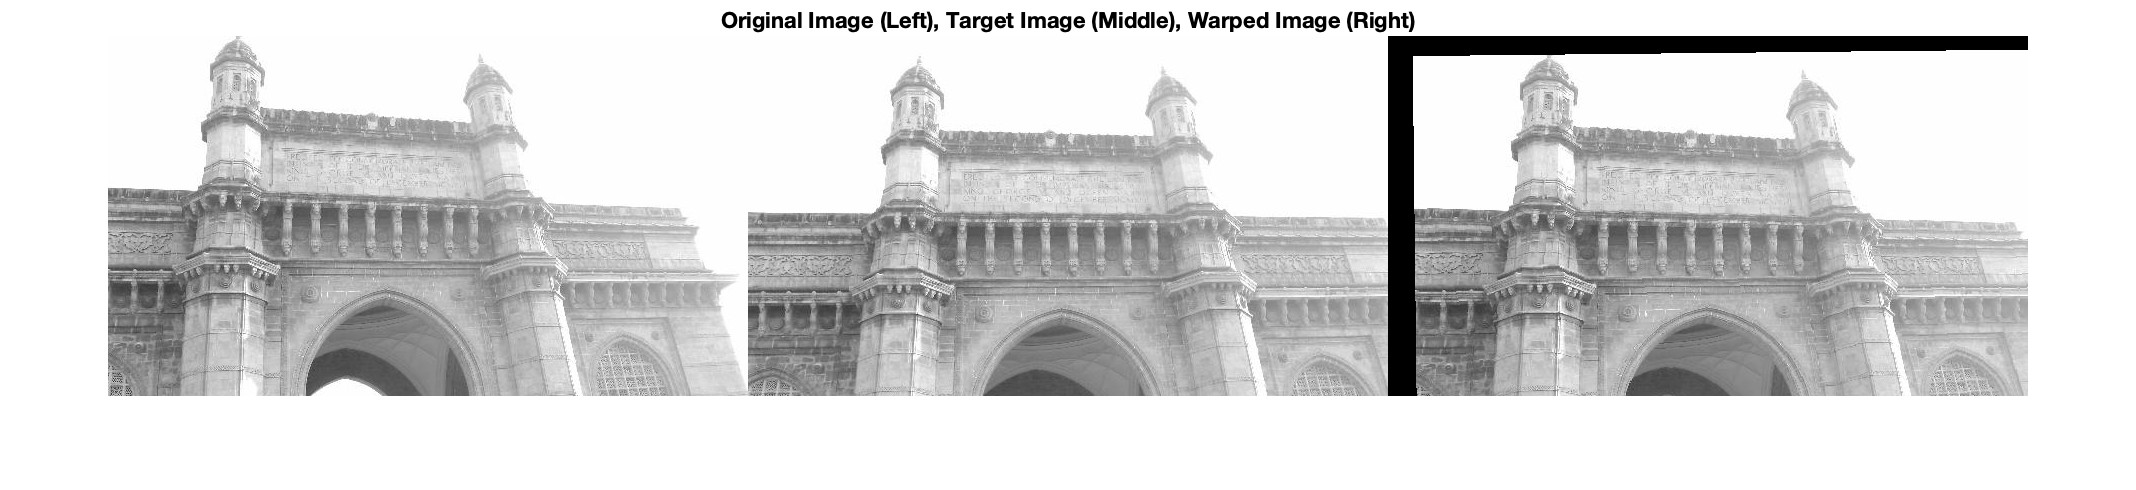
\includegraphics[width=\linewidth]{Images/Q6/nearest.jpg}
    \caption{Image warped using nearest neighbour interpolation}
\end{figure}

As we can see, the third image looks quite similar and aligned to the second image (except the black border, which comes because of out of bound values when multiplying by inv(T)).


\textbf{(d)}
In this part, we used bilinear interpolation for image warping. The approach looks similar to the previous part, but instead of mapping the intensities to nearest integral points, we consider the weighted average of all 4 neighbouring points. And the weights are the areas of the four rectangles, here is the code:
\begin{verbatim}
    for r = 1:size(im2, 1)
    for c = 1:size(im2, 2)
        originalCoords = invT * [c; r; 1];
        xOriginal = originalCoords(1);
        yOriginal = originalCoords(2);
        x1 = floor(xOriginal);
        y1 = floor(yOriginal);
        x2 = x1 + 1;
        y2 = y1 + 1;
        dx = xOriginal - x1;
        dy = yOriginal - y1;
        pixelValue = zeros(1, channels);
        if x1 >= 1 && x1 <= cols && y1 >= 1 && y1 <= rows
            pixelValue = (1-dx)*(1-dy)*double(im1(y1, x1, :));
        end
        if x2 >= 1 && x2 <= cols && y1 >= 1 && y1 <= rows
            pixelValue = pixelValue + dx*(1-dy)*double(im1(y1, x2, :));
        end
        if x1 >= 1 && x1 <= cols && y2 >= 1 && y2 <= rows
            pixelValue = pixelValue + (1-dx)*dy*double(im1(y2, x1, :));
        end
        if x2 >= 1 && x2 <= cols && y2 >= 1 && y2 <= rows
            pixelValue = pixelValue + dx*dy*double(im1(y2, x2, :));
        end
        warpedImg(r, c, :) = uint8(pixelValue);
    end
end   
\end{verbatim} 
\begin{figure}[h]
    \centering
    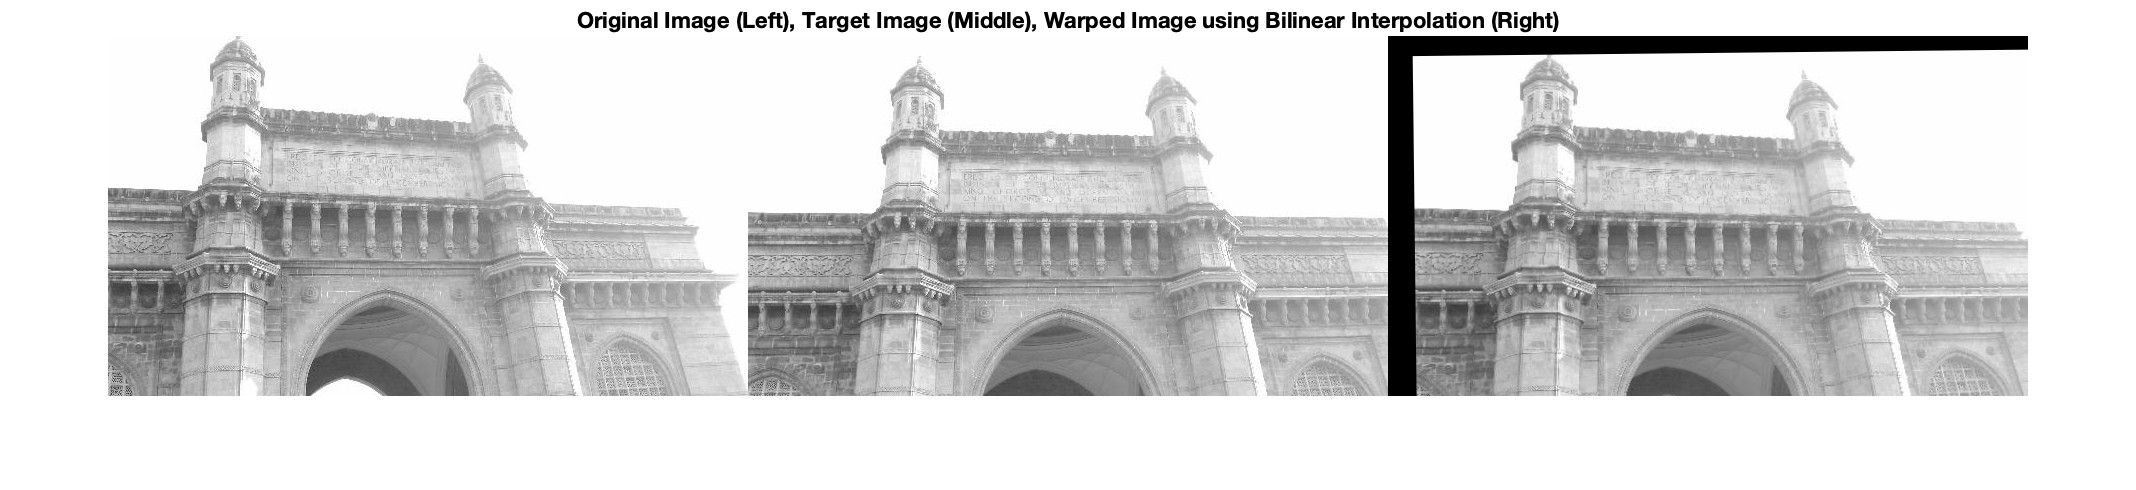
\includegraphics[width=\linewidth]{Images/Q6/bilinear.jpg}
    \caption{Image warped using bilinear interpolation}
\end{figure}
Similar to the previous case, the image aligns really well.

\textbf{(e)}
We already know that A is of the form:
\[
    \begin{bmatrix}
        x_{11} & x_{12} & x_{13} & \dots & x_{1n} \\
        y_{11} & x_{12} & y_{13} & \dots & y_{1n} \\
        1 & 1 & 1 & \dots & 1
    \end{bmatrix}
\]
and b is of the form:
\[
    \begin{bmatrix}
        x_{21} & x_{22} & x_{23} & \dots & x_{2n} \\
        y_{21} & x_{22} & y_{23} & \dots & y_{2n} \\
        1 & 1 & 1 & \dots & 1
    \end{bmatrix}
\]

It has also been given that the control points are perfectly colinear i.e. $y_{1i} = mx_{1i}+c$. 
\[b = TA\]
\[bA^T = TAA^T\]
where $A^T$ is the transpose of matrix A. We can fine $T$ if $AA^T$ is invertible. $P = AA^T$ is given by:
\[
    \begin{bmatrix}
        \sum_{i=1}^nx_{1i}^2 & a\sum_{i=1}^nx_{1i}^2 + b\sum_{i=1}^nx_{1i} & \sum_{i=1}^nx_{1i}\\
        a\sum_{i=1}^nx_{1i}^2 + b\sum_{i=1}^nx_{1i} &  a^2\sum_{i=1}^nx_{1i}^2 + 2ab\sum_{i=1}^nx_{1i} + kb^2 & a\sum_{i=1}^nx_{1i} + nb\\
        \sum_{i=1}^nx_{1i} & a\sum_{i=1}^nx_{1i} + nb & n
    \end{bmatrix}
\]

If $C_1, C_2, C_3$ are the columns of the matrix $P$, then we can see from above that $C_2 - aC_1 - bC_3 = 0$. Hence the matrix is not invertible (rank-deficient). Hence, we will not be able to find $T$ using this method. Hence, affine transformation cannot be used if we choose co-linear points.
\end{document}